\tableofcontents
\newpage

\section{Acknowledgments}

First af all I thank all the students who worked beyond my expectations, even by sending works that they were not supposed to do. Their explosion of creativity was extremely useful. Some of these contributes deserve specific mentions. First the remarkable "Creativity Exercises" of Marta Veloce, Primary Education student, that inspired chapter \ref{cap:marta}. Then Alberto Averono, teacher of a secondary school, who in a training course about coding further developed Marta's exploration. Another Primary Education student, Eleonora Aiazzi, send a moving text, "When a professor treats you as a child", who was extremely encouraging about the teaching method I was experimenting. A well experienced primary school teacher, Antonella Colombo, gave me back a wonderful documentation of Papert's syntonic learning she tried to trigger in her classroom. Her work opens the trip in chapter \ref{cap:cerchio}, from the draw of a circle to the Halley's orbit. Thanks to Piero Salonia, who corrected the proofs of the first Italian version of this manual. Finally, thanks to the beautiful world of Linux and its sharp tools  - scp, ssh, rsync, grep, find, nmap, latex, bibtex and so on - which gives true superpowers, unknown in the Graphical User Interface World - the Internet of true freedom.

\part{Basics of Logo and LibreLogo} \label{parte:manuale}

\section{Preface}
This is an English version derived from the "Piccolo Manuale di LibreLogo" that I wrote for the students of the Primary Education curriculum at the university of Florence. The manual was intended to aid the students in developing their coding activities within the "Laboratorio di Tecnologie Didattiche" (Laboratory of Educational Technologies). The programming language is LibreLogo, which is an implementation of Seymour Papert's Logo language within the Writer word processor of the LibreOffice  suite. LibreLogo is a plugin available by default in Writer since version 4.0 of LibreOffice. It has been written in Python by László Németh. The specific documentation can be found at http://librelogo.org. From there a description of all the LibreLogo commands can be downloaded in 33 different languages\footnote{The commands dictionaries can be downloaded from $https://help.libreoffice.org/Writer/LibreLogo_Toolbar$}. Apart from this, some extended documentations can be found only in Hungarian, as far as I know as of March 2018: there are a pretty technical handbook written by László Németh itself \cite{LibreLogo2} and a more classroom oriented one by Lakó Viktória \cite{LibreLogo3}. Some of the examples presented in this work have been inspired by those in  Lakó Viktória's book,  but the perspective is different here. First of all I have put  a strong emphasis on pedagogical aspects, beyond the mere technical facts, following the line of thought of Seymour Papert, as reported, for instance, in \textit{Mindstorms} \cite{Papert}. Secondly, during the couple of years since the writing of the first version of the "Piccolo Manuale di LibreLogo",  a number of reflections, exercises and hands-on practices got back from students and other sources, have been added. The overall result is a rather broad discussion of possible uses of LibreLogo, both in a vertical dimension, from primary school examples to tertiary education level exercises, and in a transverse dimension, through a variety of disciplines. Finally, this is not a true translation of the "Piccolo Manuale di LibreLogo" but an English rewriting, characterized by a somewhat more concise exposition of the same facts.

\chapter{LibreLogo} \label{cap:librelogo}

LibreLogo is the implementation of the famous Logo language within the wordprocessor Writer. Writer is the word processing application of the LibreOffice, analogously to word, which is part of MS Office suite. Logo was created by Seymour Papert in the seventies to improve the learning of math. Seymour Papert, born in South Africa in 1928, first studied math in Johannesburg and successively in Cambridge. Between 1958 and 1964 he got his PhD at the University of Geneva with Jean Piaget: interesting collaboration between a mathematician and a pedagogist. Since 1964 he was a researcher of the MIT Artificial Intelligence laboratory where, in 1967  he got the position of codirector with Marvin Minsky, a relevant scientist in the field of artificial intelligence. The laboratory is the same where Richard Stallman, father of free software, would have worked a few years later. Free software is a beautiful reality but, ironically, it is incredibly widespread and, at the same time, so few people know something about. And it is right in the school context that it should be much more diffused, because of its relevant ethic and educational features. Probably, the best known free software is the Linux operating system, but there are many more: LibreOffice, analogous of MS Office, Gimp for manipulating digital bitmap images, Inskape for vector images, Audacity for audio recorded files, OBS for streaming and screencasting, shotcut for video cutting and many others. Seymour Papert is famous for having invented Logo, a programming language for drawing by giving commands to a "Turtle". However, in the first version, conceived in the Seventies, the Turtle was a robot which was able to draw by means of a pencil.

\begin{figure}
   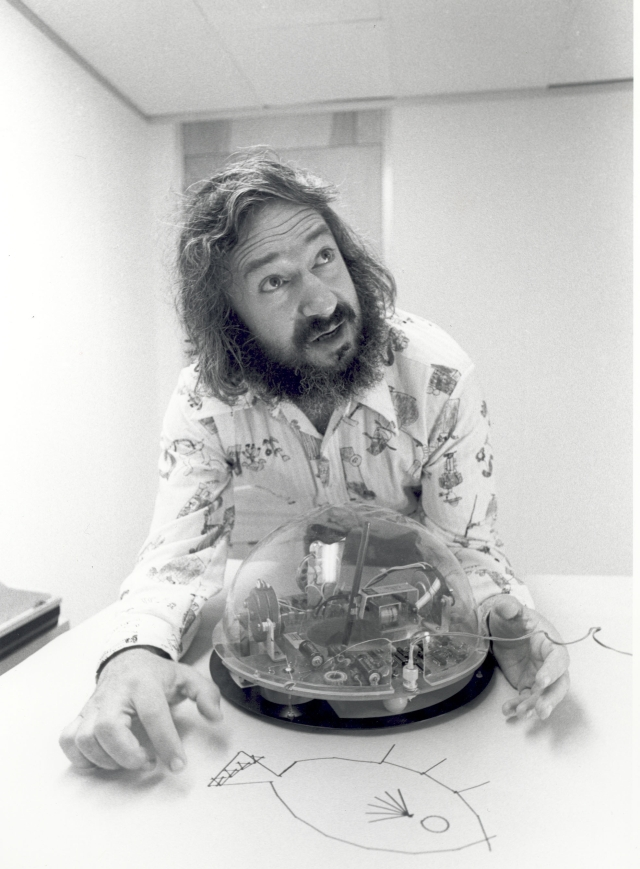
\includegraphics[width=10.0cm]{./images/librelogo/Papert-x640.jpg}
   \caption{Seymour Papert shows one of the first versions of Logo, when it was kind of a robot for draving.} 
\label{papert}
\end{figure}

When computers arrived in the homes in the 80s, Logo became a software and as such was described by Seymour Papert in  \textit{Mindstorms}. In order to understand the pedagogical value of Papert's thought, let's read this passage, taken from  \textit{Mindstorms} (pp. 7-8) \cite{Papert}:

\begin{quote} 
I take from Jean Piaget a model of children as builders of their own intellectual structures. Children seem to be innately gifted learners, acquiring long before they go to school a vast quantity of knowledge by a process I call "Piagetian learning", or "learning without being taught". For example, children learn to speak, learn the intuitive geometry needed to get around in space, and learn enough of logic and rethorics to get around parents - all this without being taught. We must ask why some learning takes place so early and spontaneously while some is delayed many years or does not happen at all without deliberately posed formal instruction. 

If we really look at the "Child as a Builder" we are on our way to an answer. All builders need materials to build with. Where I am at variance with Piaget is in the role I attribute to the surrounding cultures as a source of these materials. In some cases the culture supplies them in abundance, thus facilitating constructive Piagetian learning. For example, the fact that so many important things (knives and forks, mothers and fathers, shoes and socks) come in pairs is a "material" for the construction of an intuitive sense of number. But in many cases were Piaget would explain the slower development of a particular concept by is greater complexity or formality, I see the critical factor as the relative poverty of the culture in those materials that would make the concept simple and concrete.
\end{quote}

In the 90's Logo circulated as a program installable from a floppy disk. Once launched, it produced a black screen on which instructions could be written in sequence, one after the other. The instructions represented the movements to be given to the turtle on the screen. Then, with a special command, you could "execute" the sequence of commands, and so the turtle moved by drawing something on the screen. Logo had a great resonance as an experimental method for teaching math and a wide variety of versions have been derived, reaching to generalizations such as the current Scratch. However, it has not been widely distributed in schools and perhaps it has been more successful among kids than among teachers. Probably it was too early. Using Logo means writing code, an activity that is not part of the preparation of most teachers, including those who teach science. Today it is perhaps different, we talk a lot about \textit{coding}, even if perhaps not always with full knowledge of the facts. The situation has evolved so much that \textit{coding} can mean so many different things. Moreover, from the 1980s to the present, the variety of programming languages has grown enormously. Nowadays, among the logo derivations, Scratch is the most renowned educational programming language. Mitchel Resnick, a former student of Papert, is the project leader of Scratch and now is still following it at the MIT Media Laboratory. Scratch goes far beyond the production of graphics and allows you to create animations and video games, thus also allowing one to experiment with rather sophisticated programming techniques. Another innovative aspect is that it is structured as a web service and this has allowed the creation of a large community of living dissemination and exchange of programs. From the operational point of view, Scratch differs from Logo in that it is a visual language. The commands are in fact made up of coloured blocks that can be interlocked. The program comes out from the execution of these sequences of commands connected together, as in a puzzle. It's an attractive system that's a bit like Lego, where the instructions you give are stuck together like bricks. The joints ensure that instructions are combined only in legitimate ways, protecting against the typical and frequent spelling and syntactical errors that anyone who is writing software in the conventional text mode would encounter. Many of these languages have emerged, in addition to Scratch. The most famous are Snap!, Alice, Blockly, Android App Inventor, just to name a few. The following figure shows the difference between a text code and a visual code. The code is used to draw a square. Left the LibreLogo version and right the Snap! In Scratch this simple code would be identical. I used Snap! since I have a certain preference for this language. Snap! represents an enhancement of Scratch, which make it more similar to a generic language, while maintaining the visual form. Among these features there is the possibility of saving  the code in a standard format (XML) which is readable and editable by any text editor. For those who are used to working with software, this is a very important element. The code is not "optimal", in any sense. It is  is only intended to compare instructions in two different environments. 

\begin{figure}
   \centering
   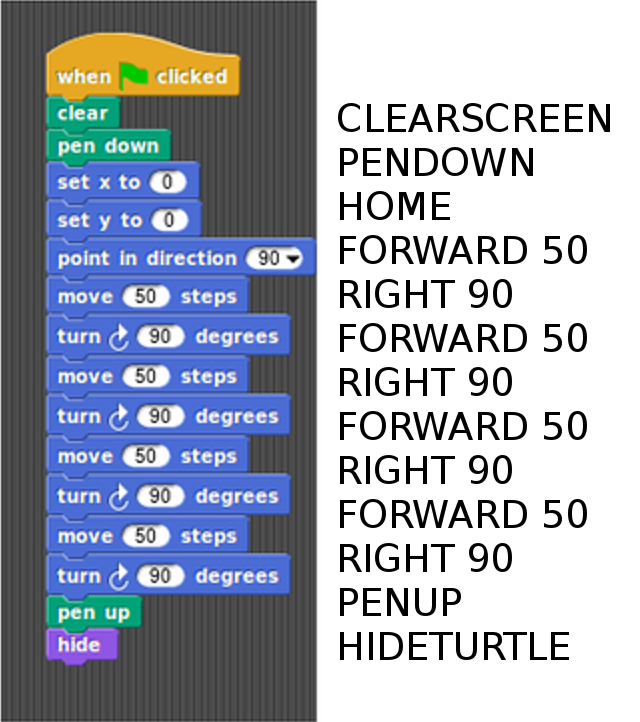
\includegraphics[width=7.5cm]{./images/librelogo/scratch-2.png}
   \label{scratch}
\end{figure}

A special feature of Scratch is that it has created a large software sharing community. This happened thanks to the fact that it was conceived as a web service, which allows the writing of programs and the possibility of running them but also the realization of a social environment for sharing and remixing the programs. Visual languages have also drawbacks. They are (apparently) easy, fun and colorful, their effectiveness would seem guaranteed but the scientific evidence is not so clear. There are in fact various studies that show that visual languages do not facilitate so much the learning of "real" languages \cite{Weintrop}. It seems that they are advantageous to understand the simplest constructs of programming but studies where the deep understanding about what a given algorithm does do not show substantial differences between visual and textual languages \cite{Weintrop2}. The research of Colleen Lewis is of particular interest. She compared the results obtained with Logo and Scratch in a class of children between 10 and 12 years \cite{Lewis}. The results showed that the learning of some specific coding constructs was facilitated by Scratch but, on the other side, the kids showed a higher level of self-esteem when introduced to programming with Logo.    

And even if in the initial phases kids prefer visual tools, later on, once they try conventional textual programming, they may perceive the limits of visual coding:

\begin{itemize}
\item as a limiting their creativity because less powerful
\item because they fill visual coding less real: "if you have to do something real, nobody will ever ask you to encode it with visual educational software" \cite{Weintrop3}
\end{itemize}

It is on the basis of such considerations that we decided to focus on the Logo language, as an introductory tool to programming. Pretty a number of Logo versions are available nowadays. We here focus on a version that is available by default in Writer, the word processing application included in the LibreOffice office suite\footnote{There is another similar project called OpenOffice. Many ask what are the differences with LibreOffice. A small history of the evolution of these two software, which have a common origin, can be found here (July 2016): http://www.navigaweb.net/2014/04/differenze-tra-openoffice-e-libreoffice.html. At present, LibreOffice is convenient because it incorporates more features and is updated more frequently.}, analogous of the widespread MS Office suite. The latter is a "proprietary product", i.e. the company that produces it sells it but without distributing the source code in clear, according to the conventional industrial model, with which the intellectual property is jealously kept secret. LibreOffice is free software, and as such is ideal for use in any educational context. Firstly, because it carries an ethical message. In fact, free software is defined by four types of freedom\footnote{Free software definition according to the free Software Foundation: https://www.gnu.org/philosophy/free-sw.en.html}:

\begin{itemize}
\item The freedom to run the program as you wish, for any purpose (freedom 0).
\item The freedom to study how the program works, and change it so it does your computing as you wish (freedom 1). Access to the source code is a precondition for this.
\item The freedom to redistribute copies so you can help your neighbor (freedom 2).
\item The freedom to distribute copies of your modified versions to others (freedom 3). By doing this you can give the whole community a chance to benefit from your changes. Access to the source code is a precondition for this.
\end{itemize}

It should be noted - on this point many people are confused - that \textit{open} \textit{source} software is different from (\textit{free} \textit{software}) since the ethical aspect is missing: open source software assumes that the source code is available in clear, but does not mention the four freedoms mentioned above and, in particular, the two specifications that characterize the ethical value of \textit{free} \textit{software}: "so as to help others" in the third freedom and "so that the whole community benefits" in the fourth freedom. Free software is developed by communities that may join together in non-profit societies. \textit{Open} \textit{source} is developed by private economic actors who adhere to the shared development paradigm because it fits well into their marketing strategies: there are companies that develop \textit{open} \textit{source} projects alongside traditional proprietary products because they find it convenient for their marketing strategies. LibreOffice's functionality can be enriched by means of many \textit{plugins}. LibreLogo is one of them and, from version 4.0 on, the LibreLogo plugin is included by \textit{default} \footnote{Di \textit{default} which means that this is the normal behavior. Those who use Linux (for Windows or Mac this problem does not exist) should take note of the following. Until the release of LibreOffice 4 excluded, install the LibreOffice extension from http://extensions.libreoffice.org/extension-center/librelogo. Instead, from version 4 on, install the Office-Library package directly, with the command \textit{sudo apt-get install library-Library}. Then you need to restart LibreOffice, if it is already open. Successively, activate the toolbar in View->Toolbars->Logo. Close and relaunch} in the program. But what does it mean to use Logo within a \textit{word} \textit{processor} like Writer, considered that this is a normal word processor while Logo is kind of a drawing language? Simple: With the LibreLogo toolbar you can produce images that are integrated into the document as if they were imported. It's a brilliant idea, due to Németh László, who reproduced the features of Logo within LibreOffice. In reality, it has further increased them, taking advantage of the Python language, with which he wrote the plugin. Using LibreLogo is very simple: you open a document in Writer, you write some code in Logo language, as you would write any other text, and then you run it by pressing the appropriate button in the LibreLogo \textit{toolbar}; if the code is correct, the turtle executes the code drawing a figure in the text, right in the middle of the page.

This design can then be managed  like any other LibreOffice graphics. The first time you launch LibreOffice the Logo toolbar is not active. Therefore you need to activate it, with the appropriate menu command: \textbf{View} $\rightarrow$ \textbf{Toolbars} $\rightarrow$ \textbf{Logo}: 

\begin{figure}[h]
   \centering
   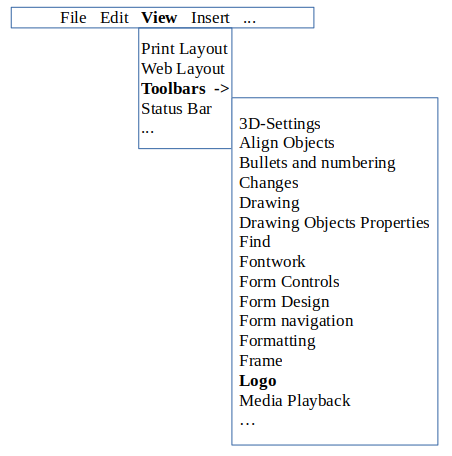
\includegraphics[width=7.5cm]{./images/librelogo/AttivazioneToolbar.png}
   \label{AttivazioneToolbar}
\end{figure}

Once this is done, you must close the program and relaunch it to see, among the other toolbars also the LibreLogo one: 

\begin{figure}[h]
   \centering
   
\includegraphics[width=7.5cm]{./images/librelogo/LibreLogoToolbar.png}
   \label{LibreLogoToolbar}
\end{figure}

where the icons have the following meanings:

\begin{center}
  \begin{tabular}{ c | l | p{5cm} }
    \hline
    
\includegraphics[width=0.75cm]{./images/librelogo/FrecciaSULO.png} & FORWARD 10 & Forward by 10 points (we will see the meaning of point successively) \\ \hline
    
\includegraphics[width=0.75cm]{./images/librelogo/FrecciagiuLO.png} & BACK 10 & Back by 10 points \\ \hline
    
\includegraphics[width=0.75cm]{./images/librelogo/Orario.png} & LEFT 15 & Left by -15 degree \\ \hline
    
\includegraphics[width=0.75cm]{./images/librelogo/Antiorario.png} & RIGHT 15 & Right by 15 degree \\ \hline
    
\includegraphics[width=0.75cm]{./images/librelogo/PlayLO.png} &  & Executes the program. Starting with version 4.3, in a newly opened document it executes a standard sampled program. \\ \hline
    
\includegraphics[width=0.75cm]{./images/librelogo/StopLO.png} &  & Stops the running program \\ \hline
    
\includegraphics[width=0.75cm]{./images/librelogo/RewindLO.png} & HOME & Brings the Turtle in its initial condition: at the center with nose up. \\ \hline
    
\includegraphics[width=0.75cm]{./images/librelogo/NewpageLO.png} & CLEARSCREEN & Cancels all the graphics - leaving the text. \\ \hline
    
\includegraphics[width=0.75cm]{./images/librelogo/220px-TextLO.png} &  & Allows to write a command and run it at once.
 \\ \hline
    
\includegraphics[width=0.75cm]{./images/librelogo/MagicwLO.png} &  &  Adjust the whole text making it uppercase. At the same time, it translates the commands in the language of the document. Currently, the dictionary file for the Italian language is set up but the commands have are still written in English. I will fix this. \\ \hline
    \hline
  \end{tabular}
\end{center}

\section{How to manage graphics in Writer}

The interaction between LibreLogo and Writer is particular for graphics. It may seem cumbersome at first but you actually have to get used to it and learn two or three rules. The probably unique feature of LibreLogo is that by running \footnote{In jargon, by "running a program" we intended to execute all its instructions. Today, with modern languages, programs are often called \textit{script}. In general, a program is a complete software and maybe also very complex. A \textit{script} tends to be a smaller, more specific fragment of code but these categories may overlap widely.} a script you get a graphic object in the same place where you have written the code, that's it in ODT document page. These objects are of "vectorial" type, that is, they are composed by a set of geometric objects. They are different from \textit{raster} or \textit{bitmap}, that consist of a matrix of pixel\footnote{A closer look at the distinction between bitmap and vector images can be found at http://https://iamarf.org/2014/02/23/elaborazione-di-immagini-tre-fatti-che-fanno-la-differenza-loptis/}. The graphic objects produced by LibreLogo are completely similar to those produced with the handwriting tools available in Writer, accessible through the special \textit{toolbar}, under the menu item \textbf{View} $\rightarrow$ \textbf{Toolbars} $\rightarrow$ \textbf{Drawing}:

\begin{figure}[h]
   \centering
   
\includegraphics[width=12.0cm]{./images/librelogo/DrawToolbar.png}
   \label{DrawToolbar}
\end{figure}

As such, drawings made with LibreLogo can be moved, copied, or saved like any other graphic object. One useful thing to understand is that such objects are often actually a composition of distinct objects. We will do many of them in this manual. To use them as a single object, use the grouping function, as follows: first, you delimit the region that includes the objects to group, by selecting \textit{pointer} 
\includegraphics[height=1em]{./images/librelogo/Pointer_LO.png} in the drawing bar and then by outlining the desired rectangular  box with the mouse and holding down the left button. Please note that the mouse cursor must be in the shape of an arrow and not the typical you have when inserting text, in the shape of a capital I, because this is where you insert text and not graphics. The fact that the graphic (and not textual) cursor is active is also understood by the fact that, at the same time, another toolbar is activated for controlling the graphics:

\begin{figure}[h]
   \centering
   
\includegraphics[width=12.0cm]{./images/librelogo/DrawToolbar2.png}
   \label{DrawToolbar2}
\end{figure}

When you select the region containing the graphic objects, icons are activated in this bar, including the icon for the grouping function: 
\includegraphics[height=1em]{./images/librelogo/RaggruppamentoLO.png}. Pressing this will group all graphic objects in the selected region into a single graphic object that can be copied elsewhere or saved. 

Another useful trick is to properly "anchor" the graphics to the document, where we have to use them. The key to determine the anchorage in the usual graphic bar is this: 
\includegraphics[height=1em]{./images/librelogo/AncoraLO.png}. By clicking on the arrow to the left of the anchor, you can select four anchor types: 1) "on page", 2) "in paragraph", 3) "in character" and 4) "as character". In the first case the graphics are associated to the page and do not move from it, in the second to a paragraph, in the third to a character and in the fourth case it behaves as if it were a character. What is the most appropriate anchorage is something that you learn from experience. Most of the graphics in this manual have been anchored "to the paragraph", except for small images that are in line with the text, as in the previous one, these are anchored "as a character".

These concern the management of graphics in Writer in general. Using LibreLogo, the only difference is that the graphics are produced through the instructions we put in the code. LibreLogo places the graphics in the middle of the first page of the document, even if the code text extends on the following pages. It may happen that the graphics overlap the text of the code itself. At first glance the result may be confusing and one can believe something wrong is going on. None of this. The graphics are produced to be used somewhere else. It is simply a matter of selecting it, as we have just described, and taking it elsewhere, in a clean page simply to see it clearly, or in some other document where it must be integrated.


